82. $\cfrac{((x^2-4)^2+y^2-2y+1)(y^2-3xy+2x^2)}{xy-2y+3x-6}=0\Leftrightarrow
\begin{cases}

((x^2-4)^2+y^2-2y+1)(y^2-3xy+2x^2)=0,\\
xy-2y+3x-6
eq0.
\end{cases}$\\$\Leftrightarrow
\begin{cases}
\left[\begin{array}{l}
(x^2-4)^2+(y-1)^2=0,\\
y(y-x)+2x(x-y)=0,
\end{array}
ight.\\
y(x-2)+3(x-2)
eq0.
\end{cases}\Leftrightarrow
\begin{cases}
\left[\begin{array}{l}
\begin{cases}
x^2-4=0,\\
y-1=0.
\end{cases}\\
(y-x)(y-2x)=0,
\end{array}
ight.\\
(x-2)(y+3)
eq0.
\end{cases}\Leftrightarrow
\begin{cases}
\left[\begin{array}{l}
\begin{cases}
x=2,\\
y=1.
\end{cases}\\
\begin{cases}
x=-2,\\
y=1.
\end{cases}\\
y=x,\\
y=2x,
\end{array}
ight.\\
x
eq2,\\
y
eq-3.
\end{cases}$
\begin{figure}[ht!]
\center{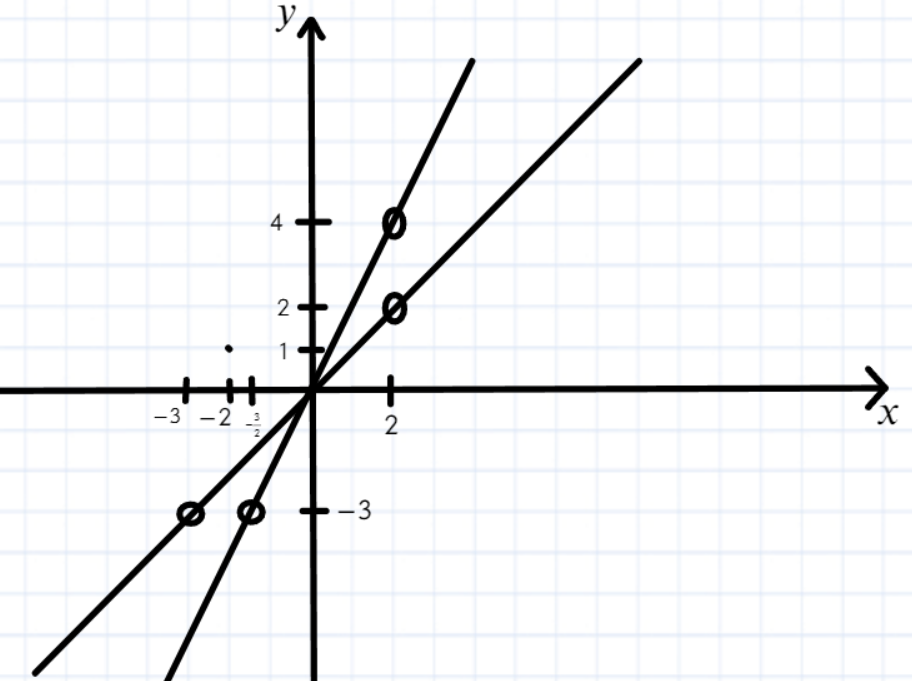
\includegraphics[scale=0.35]{gr7-82.png}}
\end{figure}
ewpage
oindent
